\documentclass[a4paper,12pt]{article}

\usepackage{times}  %Required
\usepackage{helvet}  %Required
\usepackage{courier}  %Required
\usepackage{url}  %Required
\usepackage{graphicx}  %Required

\setcounter{secnumdepth}{2} 

%%%%%%%%%%%% additional packages
%% Language and font encodings
\usepackage[english]{babel}
\usepackage[utf8x]{inputenc}
\usepackage[T1]{fontenc}

%% Useful packages
\usepackage{amsmath,amssymb,amsfonts,bbm}
\usepackage{dsfont} % for the indicator function \mathds{1}
\usepackage[svgnames]{xcolor}
\usepackage{graphicx}
\usepackage[colorinlistoftodos]{todonotes}
%\usepackage[colorlinks=true, allcolors=blue]{hyperref} % Incompatible with AAAI
%\usepackage[authoryear,round,longnamesfirst]{natbib} % Incompatible with AAAI
\usepackage{url}
\usepackage{soul}

%% Useful packages
%\usepackage{float}
%\usepackage{algpseudocode}%
\usepackage{algorithm}
\usepackage{algorithmic}
\usepackage{array}
\usepackage{indentfirst}

\usepackage{booktabs} % For formal tables
\usepackage{multirow}
\usepackage{makecell}
\usepackage{enumitem}

% Image related packages
\usepackage{verbatim}
\usepackage[export]{adjustbox}
\usepackage{subfig}
\usepackage{epstopdf}
\DeclareGraphicsExtensions{.png,.pdf,.eps,.jpg,.tif,.tiff,.ps} %MAR: moving PNG first
\graphicspath{{img//}{img/yifei-work//}{img/wordclouds//}}

%RJA added for \citet{} loved by social scientists the world over...
%\usepackage{natbib}
%but it messes with citation style already being used, so define \citet{} here:
%\newcommand{\citet}[1]{\citeauthor{#1} (\citeyear{#1})}
\newcommand{\citet}[1]{\citeauthor{#1}~\shortcite{#1}}
\newcommand{\citep}{\cite}
\newcommand{\citealp}[1]{\citeauthor{#1}~\citeyear{#1}}

%package that allows me more colors
\usepackage{soul}
\usepackage[colorinlistoftodos]{todonotes}

\definecolor{navy}{rgb}{0.1, 0.1, 0.8}
\definecolor{gray}{rgb}{0.6, 0.6, 0.6}
\definecolor{myblue}{rgb}{.8, .8, 1}
\definecolor{olive}{rgb}{0.1, 0.5, 0.1}
\definecolor{darkred}{rgb}{0.75, 0.25, 0.25}

%--------------------------------------------------

%%% comments -- ENABLE
\newcommand{\eat}[1]{}
\newcommand{\rev}[1]{{\color{navy}{#1}}}
\newcommand{\revA}[1]{{\color{navy}{#1}}}
\newcommand{\rvt}[1]{{\color{ForestGreen}{#1}}}
\newcommand{\rvr}[1]{{\color{brown}{#1}}}
\newcommand{\rvx}[1]{{\color{olive}{#1}}}
\newcommand{\oldversion}[1]{{\color{gray}{#1}}}
\newcommand{\verify}[1]{{\color{red}{#1}}}
\newcommand{\TODO}[2]{
 \hl{ {\bf #1}:~#2}
}


%% dataset names
\usepackage{xspace}
\newcommand{\debate}{{\sc \#DebateNight}\xspace}
\newcommand{\Protected}{\texttt{Protected}\xspace}
\newcommand{\Human}{\texttt{Human}\xspace}
\newcommand{\Bot}{\texttt{Bot}\xspace}
\newcommand{\Suspended}{\texttt{Suspended}\xspace}

\begin{document}


\section*{A new method for estimating influence in retweet cascades}
\label{sec:user-influence}

An {\em information cascade} $V$ of size $n$ is defined as a series of messages $v_i$ sent by user $u_i$ at time $t_i$, i.e. \rev{$V=\{v_i\}_{i=1:n}$, $v_i=(u_i, t_i)$}.
Here $v_1 = (u_1, t_1)$ is the initial message, and $v_1, \ldots, v_n$ with $t_1<\ldots<t_n$ are subsequent reposts or relays of the initial message.
In the context of Twitter, the initial message is an original tweet and the subsequent messages are retweets of that original tweet (which by definition, are also tweets).
A latent retweet diffusion graph $G=(V,E)$ has the set of tweets as its vertexes $V$, and additional edges $E=\{(v_i, v_j)\}$ that represent that the $j^{th}$ tweet is a retweet of the $i^{th}$ tweet, and respects the temporal precedence $t_i<t_j$.
Web data sources such as the Twitter API provide cascades, but not the
diffusion edges. 
Such missing data makes it challenging to measure a given user's contribution to the diffusion process.

\begin{figure}[bp]
	\newcommand\mywidth{0.19}
	\centering
	\subfloat[] {
		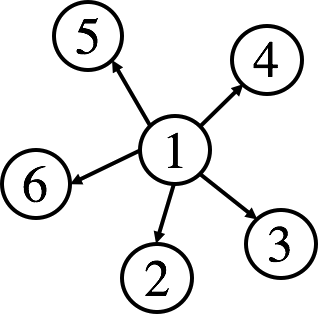
\includegraphics[width=0.12\textwidth,valign=c]{observcas}
		\vphantom{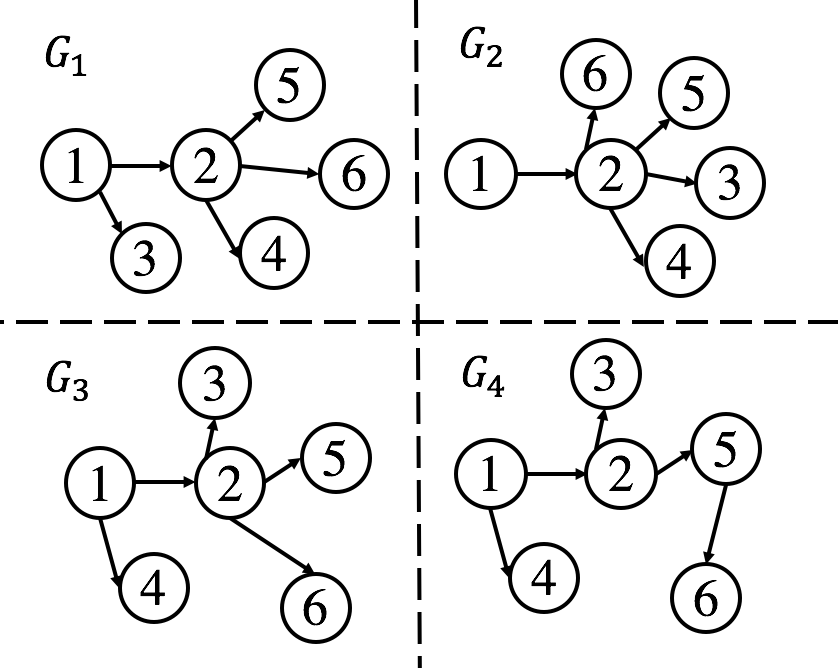
\includegraphics[height=\mywidth\textheight,valign=c]{somepossicas}}% MAR: this is here to keep the label at the same position as for the other figures.
		\label{fig:side:a}
	}
	\hspace{0.1cm}
	\subfloat[] {
		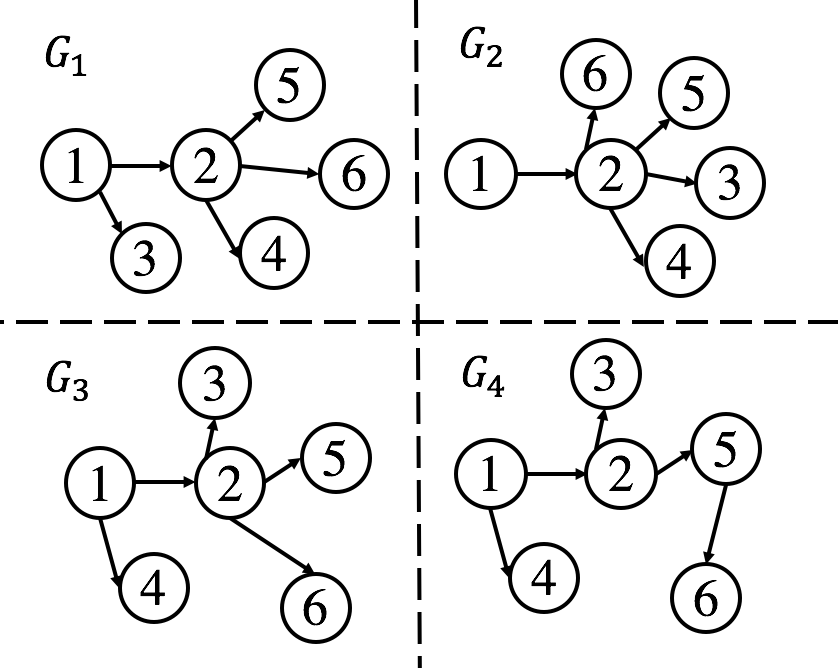
\includegraphics[height=\mywidth\textheight,valign=c]{somepossicas}
		\label{fig:side:b}
	}
	\hspace{0.1cm}
	\subfloat[] {
		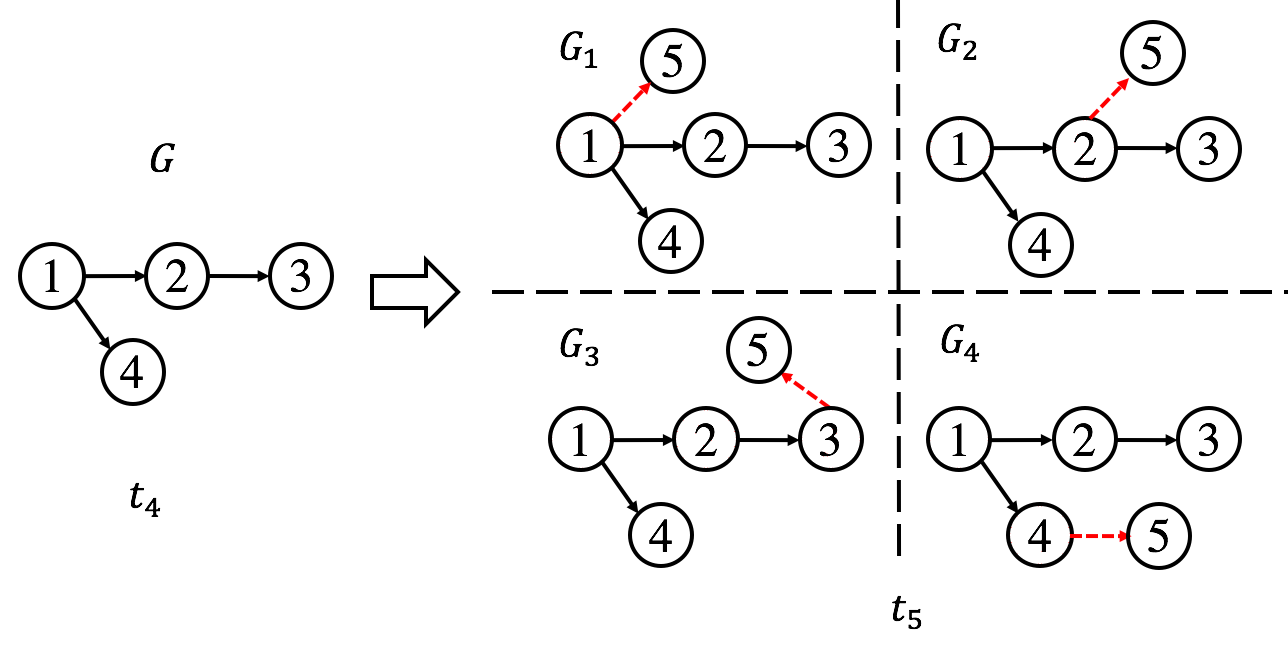
\includegraphics[height=\mywidth\textheight,valign=c]{gen_col}
		\label{fig:add-one-edge}
	}
	\caption{ 
		Modeling latent diffusions.
		\textbf{(a)} The schema of a retweet cascade as provided by the Twitter API, in which all retweets are attributed to the original tweet.
		\textbf{(b)} Four diffusion scenarios (out of 120 possible scenarios), associated with the retweet cascade in (a).
		\textbf{(c)} Intuition of the independent conditional model.
		A new node $v_5$ appears conditioned on one diffusion scenario $G$.
		Four new diffusion scenarios are generated as $v_5$ can attach to any of the existing nodes.
	}
\end{figure}

%\secmoveup
\subsection{Modeling latent diffusions}
\label{subsec:model-latent-diffusions}
%\secmoveup

\noindent\textbf{Diffusion scenarios.}
We focus on tree-structured diffusion graphs, i.e. each node $v_j$ has only one incoming link $(v_i, v_j)$, $i<j$. 
Denote the set of trees that are consistent with the temporal order in cascade $C$ as ${\cal G}$, we call each diffusion tree a \emph{diffusion scenario} $G \in {\cal G}$.
%Fig.~\ref{fig:side:a} contains a cascade visualized as a star graph, attributing subsequent tweets to the first tweet at $t_1$.
%Fig.~\ref{fig:side:b} shows four example diffusion scenarios consistent with this cascade.
The main challenge here is to estimate the influence of each user in the cascade, taking into account all possible diffusion trees.

\noindent\textbf{Probability of retweeting.}
%We define the probability of an edge $\mathds{P}(\{v_i, v_j\})$ as the likelihood that $u_j$ emitted tweet $v_j$ as a direct retweet of $v_i$.
For each tweet $v_j$, we model the probability of it being a direct descendant of each previous tweet in the same cascade as a weighted softmax function, defined by two main factors:
%% LX: the extra citations appear to be unecessary here
%as follows.
%In line with previous work~\cite{Mishra2016,Zhao2015,Shen2014}, we model two factors:
%\eat{in the likelihood of retweeting}:
firstly, users retweet \emph{fresh} content~\cite{Wu2007}.
We assume that the probability of retweeting decays exponentially with the time difference $t_j - t_i$;
secondly, users prefer to retweet influential users. 
%, known as preferential attachment~\cite{Barabasi2005,Rizoiu2017}.
We measure the local influence $m_i$ of a user $u_i$ using her number of followers~\cite{kwak2010twitter,Cha2010}.
We quantify the probability that $v_j$ is a direct retweet of $v_i$ as:
\begin{equation} \label{eq:prob-edge-mt}
	p_{ij} = \frac{m_i e^{-r({t_j-t_i})}}{\sum_{k=1}^{j-1} m_k e^{-r({t_j-t_k})}}
\end{equation}
where 
$r$ is a parameter controlling the temporal decay. 
% and
%$m_i$ is the number of followers of user $u_i$ (the user of $v_i$).
%$e^{-r({t_{b}-t_{a}})}$ express the probability decrease in exponential.
%$G$ is one diffusion scenario which user $u_b$ is added to.
%The probability of a diffusion scenario is intimately linked to the probability of an edge.
%\TODO{LX}{this seems to be event rate not probability, i.e. not normalised}

\subsection{Tweet influence in a retweet cascade}
\label{subsec:user-influence-mt}

% assumptions + difficulties
We additionally assume retweets follow {\em independent conditional diffusions} within a cascade. 
%s
This is to say that conditioned on an existing partial cascade of $j-1$ retweets $V^{(j-1)}=\{v_k\}_{k=1}^{j-1}$ whose underlying diffusion scenario is $G^{(j-1)}$, the $j^{th}$ retweet is attributed to any of the $k=1,\ldots,j-1$ prior tweets according to Eq.~\ref{eq:prob-edge-mt}, and is independent of the diffusion scenario $G^{(j-1)}$. 
%s
For example, the $5^{th}$ tweet in the cascade will incur four valid diffusion trees for each of the diffusion scenarios for 4 tweets -- this is illustrated in Fig.~\ref{fig:add-one-edge}. 
%s
This simplifying assumption is reasonable, as it indicates that each user $j$ makes up his/her own mind about whom to retweet, and that the \rev{list of previous tweets and retweets} is available to user $j$, as is true in the current user interface of Twitter.
%s
It is easy to see that under this model, the total number of valid diffusion trees for a 5-tweet cascade is $1\cdot 2\cdot 3\cdot 4=24$, and that for a cascade with $n$ tweets is $(n-1)!$.

The goal for influence estimation for each cascade is to compute the contribution $\varphi(v_i)$ of each tweet $v_i$ {\em averaging} over all independent conditional diffusion trees consistent with cascade $V$ and with edge probabilities prescribed by Eq.~\ref{eq:prob-edge-mt}. 
%s
Enumerating all valid trees and averaging is clearly computationally intractable, but the illustration in Fig.~\ref{fig:add-one-edge} lends itself to a recursive algorithm. 

\textbf{Tractable tweet influence computation}
We introduce the \emph{pair-wise influence score} $m_{ij}$, \rev{$i<j$}, which measures the influence of $v_i$ over $v_j$:
$v_i$ can influence $v_j$ both directly when $v_j$ is a retweet of $v_i$, and indirectly when a path exists from $v_i$ to $v_j$ in the underlying diffusion scenario.
Let $v_k$ be a tweet on the path from $v_i$ to $v_j$ ($i < k < j$) so that $v_j$ is a direct retweet of $v_k$.
$m_{ik}$ can be computed at the $k^{th}$ recursion step and it measures the influence of $v_i$ over $v_k$ over all possible paths starting with $v_i$ and ending with $v_k$.
Given the above independent diffusions assumption, the $m_{ij}$ can be computed using $m_{ik}$ to which we add the edge $(v_k, v_j)$.
\st{User $u_j$ can chose to retweet any of the previous tweets with probability $p_{kj}, k < j$, therefore we further weight the contribution through $v_k$ using $p_{ij}$.}
We deem a tweet to have a unit influence over itself ($m_{ii} = 1$).
This implies the following recursive relation:
\begin{equation} \label{eq:Mij-mt}
m_{ij} =
\left\{
\begin{array}{ll}
	\sum^{j-1}_{k=i} m_{ik}p_{kj} &,i < j \\
	1 & ,i = j \\
	0 & ,i > j.
\end{array}
\right.
\end{equation}

Naturally, $\varphi(v_i)$ the total influence of node $v_i$ is the sum of $m_{ij}, j > i$ the pair-wise influence score of $v_i$ over all subsequent nodes $v_j$. 
The recursive algorithm has three steps. 
\begin{enumerate}
	\item {\bf Initialization.} $m_{ij}=0$ for $i, j=1,\ldots,n, j \neq i$, and $m_{ii} = 1$ for $i=1,\ldots,n$;
	\item {\bf Recursion.} For $j=2, \ldots, n$;
	\begin{enumerate}
		\item For $k=1, \ldots, j-1$, compute $p_{kj}$ using Eq.~\eqref{eq:prob-edge-mt};
		\item For $i=1, \ldots, j-1$, \rev{$m_{ij} = \sum_{k=i}^{j-1} m_{ik}p_{kj}$};
	\end{enumerate}
	\item {\bf Termination.} Output $\varphi_i= \sum_{k=i+1}^n m_{ik}$, for $i=1,\ldots,n$. 
\end{enumerate}


\rev{
\subsection{Normalising influences among diffusion trees}

\noindent{\bf Claim 1:} Under the recursion recipe above, the probability of all $n$-node diffusion trees (i.e. valid diffusion scenarios) sums to 1. 

A proof can be obtained by recursion. Sketch: 
Denote the set of $n$-node trees as ${\cal G}_n$, the number of trees $|{\cal G}_n|$, an arbitrary tree in this set ${\cal T}_i \in {\cal G}_n$. Under the conditional independent diffusion model, the probability of a certain tree $P({\cal T}_i)$ is the product of all its edge probabilities. One can show that:
\begin{align}
\sum_{i=1}^{|{\cal G}_n|} P({\cal T}_i) = \sum_{j=1}^{|{\cal G}_{n-1}|} P({\cal T}_j)  \sum_{k=1}^{n-1} p_{kn}
\label{eq:treesum}
\end{align}
The first sum is 1 by recursion, the second term sums to 1 by Equation~\ref{eq:prob-edge-mt}. 

This result implies that in an $n$-node diffusion, the credit for creating $n-1$ retweets should be proportion distributed to each tree according to its own probability, and to each node according to their respective contribution to all the trees. 

\noindent{\bf TODO: @Rohit to write out a full proof?}

\vspace{1mm}
\noindent{\bf Question 2:} What is the correct normalisation for the contribution of a user $i$ ?  i.e. for a cascade of n tweets, how many {\em credit} in total are being distributed across all users who participated.
%is $\varphi_i (n-1)$. 
%This is from the nominal similarity between the recursion in Eq~\ref{eq:Mij-mt} and Eq~\ref{eq:treesum}. 

\noindent{\bf TODO: @Rohit to investigate and let us know?}

\TODO{MAR}{I would actually suspect that $\varphi_i = \varphi(u_i) \in [1, \infty)$. In other words, we don't need any normalization, since $\varphi$ is \emph{the expected number of retweets} -- i.e. tweets downstream in retweet tree.}
}


\rev{
\subsection{A probabilistic interpretation}

Recall the familiar marked Hawkes point process with exponential kernel.
$$\lambda(t) = \mu + \sum_{t_i < t} m_i e^{-r(t-t_i)}, ~\mu=0$$

For the $j-th$ event happening at $t_j$, $j>i$, the probability of event $j$ being triggered by event $i$ is described by Equation~\ref{eq:prob-edge-mt} [Luis and Moller, other literature]. 

This observation leads to several avenues for further inquiry:

\begin{itemize}
\item One can now write out the likelihood of a diffusion cascade using the underlying Hawkes process. This enables maximum likelihood estimation for parameter $r$ -- i.e. it is now a parameter rather than hyper-parameter, and can be estimated for one cascade, a group of cascades, or the whole dataset. 
\item One can also investigate alternative parameterisations, or more than one learnable parameters for diffusion cascades. For example:
\begin{itemize}
\item Scaling user influence logarithmically may better suit the phenomena that the number of followers is long-tailed, and that the order of magnitude matters. 
$$\lambda(t) = \sum_{t_i < t} \log(m_i) e^{-r(t-t_i)}$$
\item Alternatively, one can learn a power warping parameter for influence. 
$$\lambda(t) = \sum_{t_i < t} \beta\log(m_i) e^{-r(t-t_i)}$$
\item One can also substitute the exponential kernel with power-law, neural net, or other alternatives to see which one explains the cascade better. 
\end{itemize}
\item The Hawkes process can readily explain diffusion {\em constellations}. If $\mu \neq 0$, then a Hawkes process with immigrants can explain a set of cascades about the same URL. 
\end{itemize}

}


{ %\small
\bibliography{paper}
\bibliographystyle{apalike}
}

\end{document}